% Created by tikzDevice version 0.6.1 on 2011-06-26 17:49:00
% !TEX encoding = UTF-8 Unicode
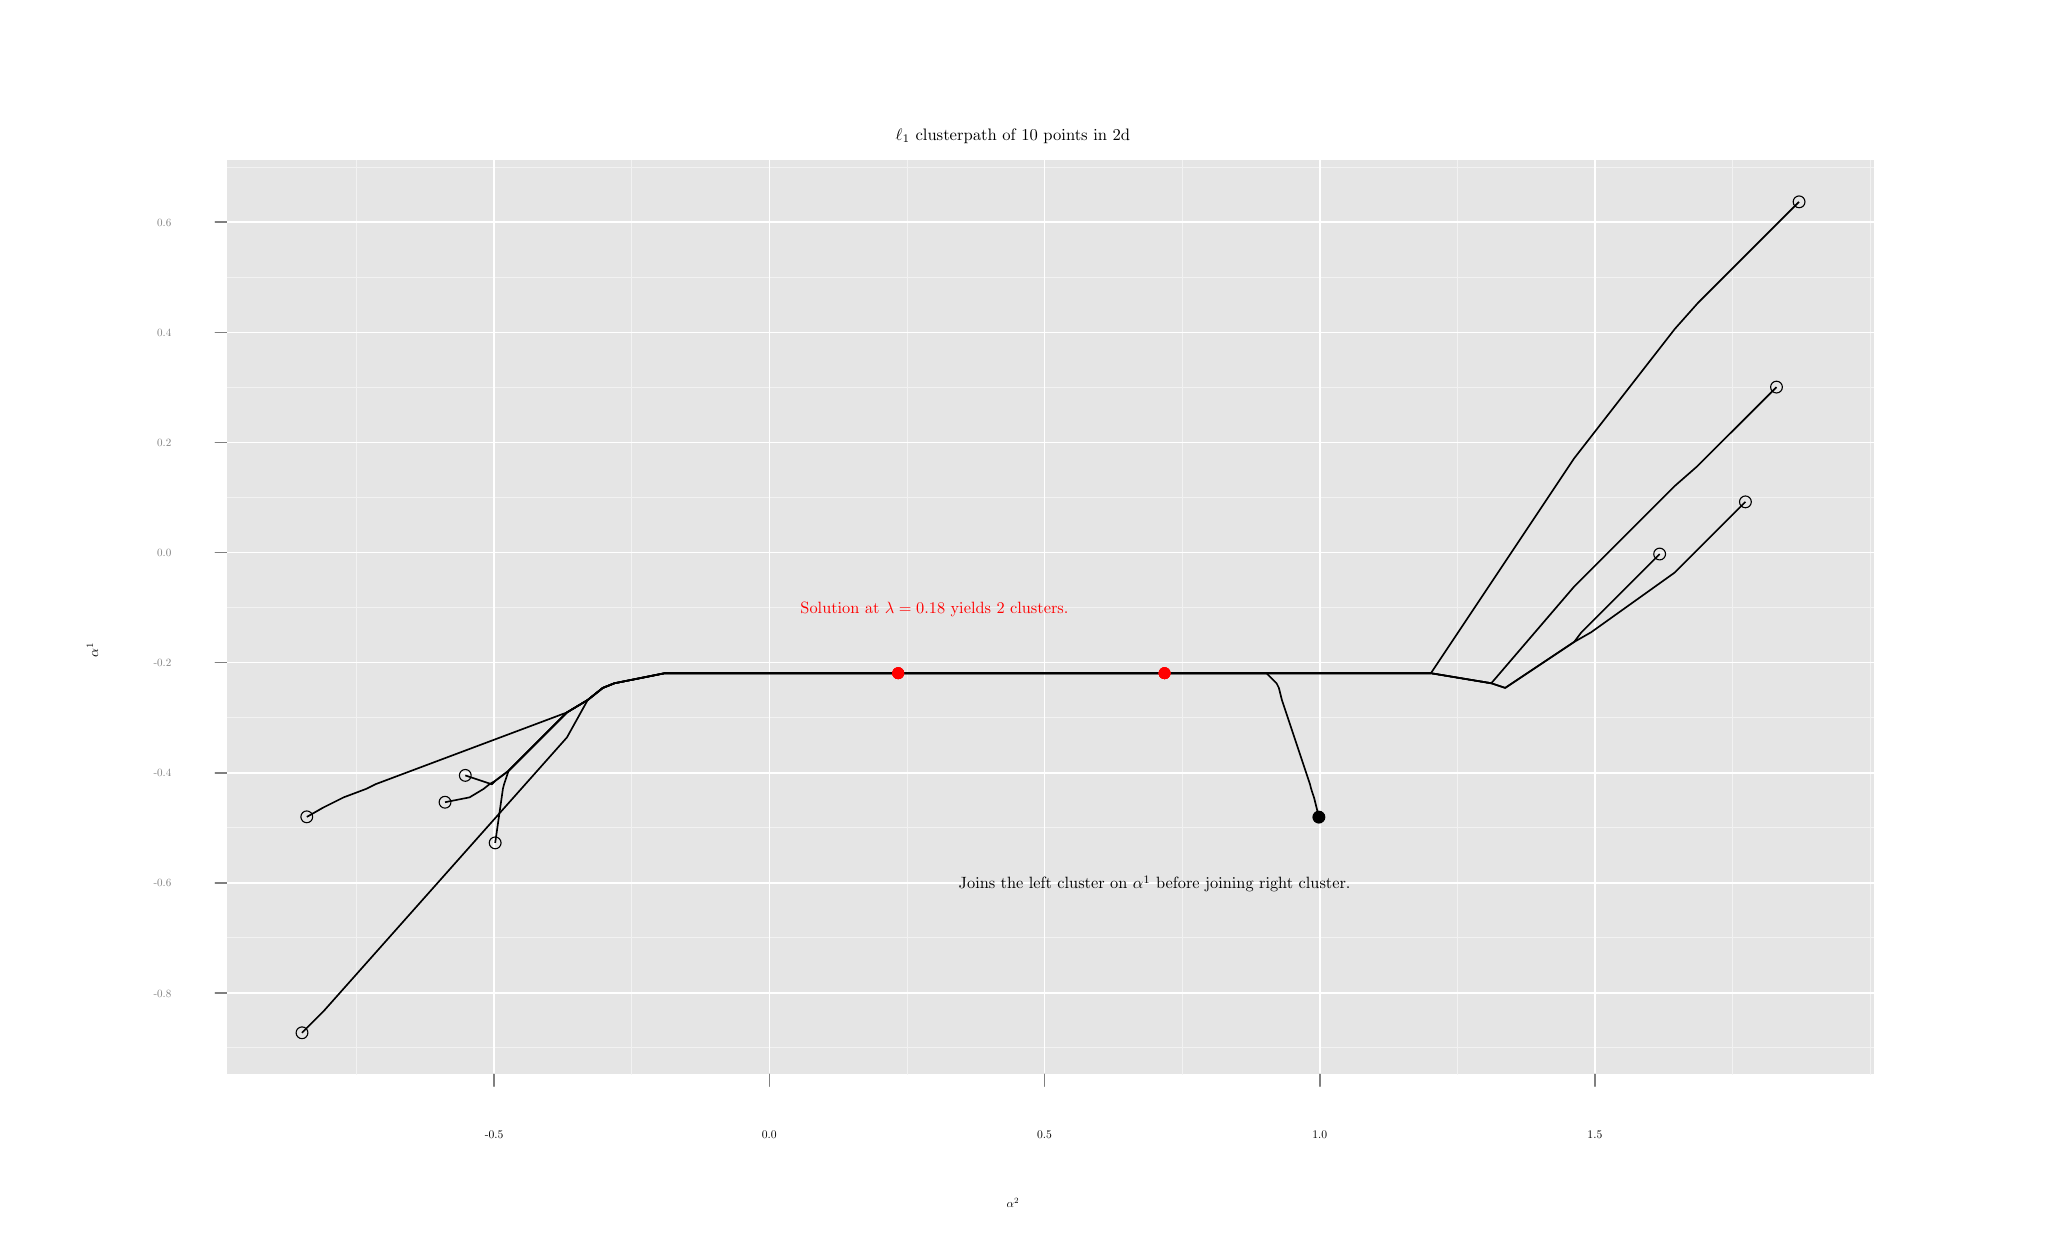
\begin{tikzpicture}[x=1pt,y=1pt]
\definecolor[named]{drawColor}{rgb}{0.00,0.00,0.00}
\definecolor[named]{fillColor}{rgb}{1.00,1.00,1.00}
\fill[color=fillColor,] (0,0) rectangle (722.70,433.62);
\begin{scope}
\path[clip] (  0.00,  0.00) rectangle (722.70,433.62);
\end{scope}
\begin{scope}
\path[clip] (  0.00,  0.00) rectangle (722.70,433.62);
\end{scope}
\begin{scope}
\path[clip] (  0.00,  0.00) rectangle (722.70,433.62);
\end{scope}
\begin{scope}
\path[clip] (  0.00,  0.00) rectangle (722.70,433.62);
\end{scope}
\begin{scope}
\path[clip] (  0.00,  0.00) rectangle (722.70,433.62);
\end{scope}
\begin{scope}
\path[clip] (  0.00,  0.00) rectangle (722.70,433.62);
\end{scope}
\begin{scope}
\path[clip] (  0.00,  0.00) rectangle (722.70,433.62);
\end{scope}
\begin{scope}
\path[clip] (  0.00,  0.00) rectangle (722.70,433.62);
\end{scope}
\begin{scope}
\path[clip] (  0.00,  0.00) rectangle (722.70,433.62);
\definecolor[named]{fillColor}{rgb}{1.00,1.00,1.00}

\draw[fill=fillColor,draw opacity=0.00,] (  0.00,  0.00) rectangle (722.70,433.62);
\end{scope}
\begin{scope}
\path[clip] (  0.00,  0.00) rectangle (722.70,433.62);
\definecolor[named]{drawColor}{rgb}{0.00,0.00,0.00}

\node[color=drawColor,anchor=base,inner sep=0pt, outer sep=0pt, scale=  0.60] at (356.02,392.92) {$\ell_1$ clusterpath of 10 points in 2d%
};
\end{scope}
\begin{scope}
\path[clip] (  0.00,  0.00) rectangle (722.70,433.62);
\definecolor[named]{drawColor}{rgb}{0.00,0.00,0.00}

\node[color=drawColor,anchor=base,inner sep=0pt, outer sep=0pt, scale=  0.42] at (356.02,  7.23) {$\alpha^2$\hspace{2in}%
};
\end{scope}
\begin{scope}
\path[clip] (  0.00,  0.00) rectangle (722.70,433.62);
\definecolor[named]{drawColor}{rgb}{0.00,0.00,0.00}

\node[rotate= 90.00,color=drawColor,anchor=base,inner sep=0pt, outer sep=0pt, scale=  0.50] at ( 25.48,208.89) {$\alpha^1$%
};
\end{scope}
\begin{scope}
\path[clip] (  0.00,  0.00) rectangle (722.70,433.62);
\end{scope}
\begin{scope}
\path[clip] ( 44.91,385.70) rectangle ( 72.08,385.70);
\end{scope}
\begin{scope}
\path[clip] (  0.00,  0.00) rectangle (722.70,433.62);
\end{scope}
\begin{scope}
\path[clip] ( 44.91,385.70) rectangle ( 72.08,385.70);
\end{scope}
\begin{scope}
\path[clip] (  0.00,  0.00) rectangle (722.70,433.62);
\end{scope}
\begin{scope}
\path[clip] (  0.00,  0.00) rectangle (722.70,433.62);
\end{scope}
\begin{scope}
\path[clip] (  0.00,  0.00) rectangle (722.70,433.62);
\end{scope}
\begin{scope}
\path[clip] ( 44.91, 55.41) rectangle ( 72.08, 55.41);
\end{scope}
\begin{scope}
\path[clip] (  0.00,  0.00) rectangle (722.70,433.62);
\end{scope}
\begin{scope}
\path[clip] ( 44.91, 32.08) rectangle ( 72.08, 55.41);
\end{scope}
\begin{scope}
\path[clip] (  0.00,  0.00) rectangle (722.70,433.62);
\end{scope}
\begin{scope}
\path[clip] ( 44.91, 32.08) rectangle ( 72.08, 32.08);
\end{scope}
\begin{scope}
\path[clip] (  0.00,  0.00) rectangle (722.70,433.62);
\end{scope}
\begin{scope}
\path[clip] ( 72.08,385.70) rectangle ( 72.08,385.70);
\end{scope}
\begin{scope}
\path[clip] (  0.00,  0.00) rectangle (722.70,433.62);
\end{scope}
\begin{scope}
\path[clip] ( 72.08,385.70) rectangle ( 72.08,385.70);
\end{scope}
\begin{scope}
\path[clip] (  0.00,  0.00) rectangle (722.70,433.62);
\end{scope}
\begin{scope}
\path[clip] ( 72.08, 55.41) rectangle ( 72.08,385.70);
\end{scope}
\begin{scope}
\path[clip] (  0.00,  0.00) rectangle (722.70,433.62);
\end{scope}
\begin{scope}
\path[clip] ( 72.08, 55.41) rectangle ( 72.08, 55.41);
\end{scope}
\begin{scope}
\path[clip] (  0.00,  0.00) rectangle (722.70,433.62);
\end{scope}
\begin{scope}
\path[clip] ( 72.08, 32.08) rectangle ( 72.08, 55.41);
\end{scope}
\begin{scope}
\path[clip] (  0.00,  0.00) rectangle (722.70,433.62);
\end{scope}
\begin{scope}
\path[clip] ( 72.08, 32.08) rectangle ( 72.08, 32.08);
\end{scope}
\begin{scope}
\path[clip] (  0.00,  0.00) rectangle (722.70,433.62);
\end{scope}
\begin{scope}
\path[clip] ( 72.08,385.70) rectangle (667.14,385.70);
\end{scope}
\begin{scope}
\path[clip] (  0.00,  0.00) rectangle (722.70,433.62);
\end{scope}
\begin{scope}
\path[clip] ( 72.08,385.70) rectangle (667.14,385.70);
\end{scope}
\begin{scope}
\path[clip] (  0.00,  0.00) rectangle (722.70,433.62);
\end{scope}
\begin{scope}
\path[clip] ( 72.08, 55.41) rectangle (667.14,385.70);
\end{scope}
\begin{scope}
\path[clip] (  0.00,  0.00) rectangle (722.70,433.62);
\end{scope}
\begin{scope}
\path[clip] ( 72.08, 55.41) rectangle (667.14, 55.41);
\end{scope}
\begin{scope}
\path[clip] (  0.00,  0.00) rectangle (722.70,433.62);
\end{scope}
\begin{scope}
\path[clip] (  0.00,  0.00) rectangle (722.70,433.62);
\end{scope}
\begin{scope}
\path[clip] (  0.00,  0.00) rectangle (722.70,433.62);
\end{scope}
\begin{scope}
\path[clip] ( 72.08, 32.08) rectangle (667.14, 32.08);
\end{scope}
\begin{scope}
\path[clip] (  0.00,  0.00) rectangle (722.70,433.62);
\end{scope}
\begin{scope}
\path[clip] (667.14,385.70) rectangle (667.14,385.70);
\end{scope}
\begin{scope}
\path[clip] (  0.00,  0.00) rectangle (722.70,433.62);
\end{scope}
\begin{scope}
\path[clip] (667.14,385.70) rectangle (667.14,385.70);
\end{scope}
\begin{scope}
\path[clip] (  0.00,  0.00) rectangle (722.70,433.62);
\end{scope}
\begin{scope}
\path[clip] (667.14, 55.41) rectangle (667.14,385.70);
\end{scope}
\begin{scope}
\path[clip] (  0.00,  0.00) rectangle (722.70,433.62);
\end{scope}
\begin{scope}
\path[clip] (667.14, 55.41) rectangle (667.14, 55.41);
\end{scope}
\begin{scope}
\path[clip] (  0.00,  0.00) rectangle (722.70,433.62);
\end{scope}
\begin{scope}
\path[clip] (667.14, 32.08) rectangle (667.14, 55.41);
\end{scope}
\begin{scope}
\path[clip] (  0.00,  0.00) rectangle (722.70,433.62);
\end{scope}
\begin{scope}
\path[clip] (667.14, 32.08) rectangle (667.14, 32.08);
\end{scope}
\begin{scope}
\path[clip] (  0.00,  0.00) rectangle (722.70,433.62);
\end{scope}
\begin{scope}
\path[clip] (667.14,385.70) rectangle (667.14,385.70);
\end{scope}
\begin{scope}
\path[clip] (  0.00,  0.00) rectangle (722.70,433.62);
\end{scope}
\begin{scope}
\path[clip] (667.14,385.70) rectangle (667.14,385.70);
\end{scope}
\begin{scope}
\path[clip] (  0.00,  0.00) rectangle (722.70,433.62);
\end{scope}
\begin{scope}
\path[clip] (667.14, 55.41) rectangle (667.14,385.70);
\end{scope}
\begin{scope}
\path[clip] (  0.00,  0.00) rectangle (722.70,433.62);
\end{scope}
\begin{scope}
\path[clip] (667.14, 55.41) rectangle (667.14, 55.41);
\end{scope}
\begin{scope}
\path[clip] (  0.00,  0.00) rectangle (722.70,433.62);
\end{scope}
\begin{scope}
\path[clip] (667.14, 32.08) rectangle (667.14, 55.41);
\end{scope}
\begin{scope}
\path[clip] (  0.00,  0.00) rectangle (722.70,433.62);
\end{scope}
\begin{scope}
\path[clip] (667.14, 32.08) rectangle (667.14, 32.08);
\end{scope}
\begin{scope}
\path[clip] (  0.00,  0.00) rectangle (722.70,433.62);
\end{scope}
\begin{scope}
\path[clip] (667.14,385.70) rectangle (667.14,385.70);
\end{scope}
\begin{scope}
\path[clip] (  0.00,  0.00) rectangle (722.70,433.62);
\end{scope}
\begin{scope}
\path[clip] (667.14,385.70) rectangle (667.14,385.70);
\end{scope}
\begin{scope}
\path[clip] (  0.00,  0.00) rectangle (722.70,433.62);
\end{scope}
\begin{scope}
\path[clip] (667.14, 55.41) rectangle (667.14,385.70);
\end{scope}
\begin{scope}
\path[clip] (  0.00,  0.00) rectangle (722.70,433.62);
\end{scope}
\begin{scope}
\path[clip] (667.14, 55.41) rectangle (667.14, 55.41);
\end{scope}
\begin{scope}
\path[clip] (  0.00,  0.00) rectangle (722.70,433.62);
\end{scope}
\begin{scope}
\path[clip] (667.14, 32.08) rectangle (667.14, 55.41);
\end{scope}
\begin{scope}
\path[clip] (  0.00,  0.00) rectangle (722.70,433.62);
\end{scope}
\begin{scope}
\path[clip] (667.14, 32.08) rectangle (667.14, 32.08);
\end{scope}
\begin{scope}
\path[clip] (  0.00,  0.00) rectangle (722.70,433.62);
\end{scope}
\begin{scope}
\path[clip] ( 44.91,385.70) rectangle ( 72.08,385.70);
\end{scope}
\begin{scope}
\path[clip] (  0.00,  0.00) rectangle (722.70,433.62);
\end{scope}
\begin{scope}
\path[clip] ( 44.91,385.70) rectangle ( 72.08,385.70);
\end{scope}
\begin{scope}
\path[clip] (  0.00,  0.00) rectangle (722.70,433.62);
\end{scope}
\begin{scope}
\path[clip] (  0.00,  0.00) rectangle (722.70,433.62);
\definecolor[named]{drawColor}{rgb}{0.50,0.50,0.50}

\node[color=drawColor,anchor=base east,inner sep=0pt, outer sep=0pt, scale=  0.40] at ( 51.92, 83.34) {-0.8%
};

\node[color=drawColor,anchor=base east,inner sep=0pt, outer sep=0pt, scale=  0.40] at ( 51.92,123.12) {-0.6%
};

\node[color=drawColor,anchor=base east,inner sep=0pt, outer sep=0pt, scale=  0.40] at ( 51.92,162.89) {-0.4%
};

\node[color=drawColor,anchor=base east,inner sep=0pt, outer sep=0pt, scale=  0.40] at ( 51.92,202.67) {-0.2%
};

\node[color=drawColor,anchor=base east,inner sep=0pt, outer sep=0pt, scale=  0.40] at ( 51.92,242.44) {0.0%
};

\node[color=drawColor,anchor=base east,inner sep=0pt, outer sep=0pt, scale=  0.40] at ( 51.92,282.22) {0.2%
};

\node[color=drawColor,anchor=base east,inner sep=0pt, outer sep=0pt, scale=  0.40] at ( 51.92,321.99) {0.4%
};

\node[color=drawColor,anchor=base east,inner sep=0pt, outer sep=0pt, scale=  0.40] at ( 51.92,361.77) {0.6%
};
\end{scope}
\begin{scope}
\path[clip] (  0.00,  0.00) rectangle (722.70,433.62);
\definecolor[named]{drawColor}{rgb}{0.50,0.50,0.50}

\draw[color=drawColor,line width= 0.6pt,line cap=round,line join=round,fill opacity=0.00,] ( 67.82, 84.86) -- ( 72.08, 84.86);

\draw[color=drawColor,line width= 0.6pt,line cap=round,line join=round,fill opacity=0.00,] ( 67.82,124.64) -- ( 72.08,124.64);

\draw[color=drawColor,line width= 0.6pt,line cap=round,line join=round,fill opacity=0.00,] ( 67.82,164.41) -- ( 72.08,164.41);

\draw[color=drawColor,line width= 0.6pt,line cap=round,line join=round,fill opacity=0.00,] ( 67.82,204.19) -- ( 72.08,204.19);

\draw[color=drawColor,line width= 0.6pt,line cap=round,line join=round,fill opacity=0.00,] ( 67.82,243.96) -- ( 72.08,243.96);

\draw[color=drawColor,line width= 0.6pt,line cap=round,line join=round,fill opacity=0.00,] ( 67.82,283.74) -- ( 72.08,283.74);

\draw[color=drawColor,line width= 0.6pt,line cap=round,line join=round,fill opacity=0.00,] ( 67.82,323.51) -- ( 72.08,323.51);

\draw[color=drawColor,line width= 0.6pt,line cap=round,line join=round,fill opacity=0.00,] ( 67.82,363.29) -- ( 72.08,363.29);
\end{scope}
\begin{scope}
\path[clip] (  0.00,  0.00) rectangle (722.70,433.62);
\end{scope}
\begin{scope}
\path[clip] (  0.00,  0.00) rectangle (722.70,433.62);
\end{scope}
\begin{scope}
\path[clip] (  0.00,  0.00) rectangle (722.70,433.62);
\end{scope}
\begin{scope}
\path[clip] ( 44.91, 55.41) rectangle ( 72.08, 55.41);
\end{scope}
\begin{scope}
\path[clip] (  0.00,  0.00) rectangle (722.70,433.62);
\end{scope}
\begin{scope}
\path[clip] ( 44.91, 32.08) rectangle ( 72.08, 55.41);
\end{scope}
\begin{scope}
\path[clip] (  0.00,  0.00) rectangle (722.70,433.62);
\end{scope}
\begin{scope}
\path[clip] ( 44.91, 32.08) rectangle ( 72.08, 32.08);
\end{scope}
\begin{scope}
\path[clip] (  0.00,  0.00) rectangle (722.70,433.62);
\end{scope}
\begin{scope}
\path[clip] ( 72.08,385.70) rectangle ( 72.08,385.70);
\end{scope}
\begin{scope}
\path[clip] (  0.00,  0.00) rectangle (722.70,433.62);
\end{scope}
\begin{scope}
\path[clip] ( 72.08,385.70) rectangle ( 72.08,385.70);
\end{scope}
\begin{scope}
\path[clip] (  0.00,  0.00) rectangle (722.70,433.62);
\end{scope}
\begin{scope}
\path[clip] ( 72.08, 55.41) rectangle ( 72.08,385.70);
\end{scope}
\begin{scope}
\path[clip] (  0.00,  0.00) rectangle (722.70,433.62);
\end{scope}
\begin{scope}
\path[clip] ( 72.08, 55.41) rectangle ( 72.08, 55.41);
\end{scope}
\begin{scope}
\path[clip] (  0.00,  0.00) rectangle (722.70,433.62);
\end{scope}
\begin{scope}
\path[clip] ( 72.08, 32.08) rectangle ( 72.08, 55.41);
\end{scope}
\begin{scope}
\path[clip] (  0.00,  0.00) rectangle (722.70,433.62);
\end{scope}
\begin{scope}
\path[clip] ( 72.08, 32.08) rectangle ( 72.08, 32.08);
\end{scope}
\begin{scope}
\path[clip] (  0.00,  0.00) rectangle (722.70,433.62);
\end{scope}
\begin{scope}
\path[clip] ( 72.08,385.70) rectangle (667.14,385.70);
\end{scope}
\begin{scope}
\path[clip] (  0.00,  0.00) rectangle (722.70,433.62);
\end{scope}
\begin{scope}
\path[clip] ( 72.08,385.70) rectangle (667.14,385.70);
\end{scope}
\begin{scope}
\path[clip] (  0.00,  0.00) rectangle (722.70,433.62);
\end{scope}
\begin{scope}
\path[clip] ( 72.08, 55.41) rectangle (667.14,385.70);
\definecolor[named]{fillColor}{rgb}{0.90,0.90,0.90}

\draw[fill=fillColor,draw opacity=0.00,] ( 72.08, 55.41) rectangle (667.14,385.70);
\definecolor[named]{drawColor}{rgb}{0.95,0.95,0.95}

\draw[color=drawColor,line width= 0.3pt,line cap=round,line join=round,fill opacity=0.00,] ( 72.08, 64.97) --
	(667.14, 64.97);

\draw[color=drawColor,line width= 0.3pt,line cap=round,line join=round,fill opacity=0.00,] ( 72.08, 84.86) --
	(667.14, 84.86);

\draw[color=drawColor,line width= 0.3pt,line cap=round,line join=round,fill opacity=0.00,] ( 72.08,104.75) --
	(667.14,104.75);

\draw[color=drawColor,line width= 0.3pt,line cap=round,line join=round,fill opacity=0.00,] ( 72.08,124.64) --
	(667.14,124.64);

\draw[color=drawColor,line width= 0.3pt,line cap=round,line join=round,fill opacity=0.00,] ( 72.08,144.52) --
	(667.14,144.52);

\draw[color=drawColor,line width= 0.3pt,line cap=round,line join=round,fill opacity=0.00,] ( 72.08,164.41) --
	(667.14,164.41);

\draw[color=drawColor,line width= 0.3pt,line cap=round,line join=round,fill opacity=0.00,] ( 72.08,184.30) --
	(667.14,184.30);

\draw[color=drawColor,line width= 0.3pt,line cap=round,line join=round,fill opacity=0.00,] ( 72.08,204.19) --
	(667.14,204.19);

\draw[color=drawColor,line width= 0.3pt,line cap=round,line join=round,fill opacity=0.00,] ( 72.08,224.08) --
	(667.14,224.08);

\draw[color=drawColor,line width= 0.3pt,line cap=round,line join=round,fill opacity=0.00,] ( 72.08,243.96) --
	(667.14,243.96);

\draw[color=drawColor,line width= 0.3pt,line cap=round,line join=round,fill opacity=0.00,] ( 72.08,263.85) --
	(667.14,263.85);

\draw[color=drawColor,line width= 0.3pt,line cap=round,line join=round,fill opacity=0.00,] ( 72.08,283.74) --
	(667.14,283.74);

\draw[color=drawColor,line width= 0.3pt,line cap=round,line join=round,fill opacity=0.00,] ( 72.08,303.63) --
	(667.14,303.63);

\draw[color=drawColor,line width= 0.3pt,line cap=round,line join=round,fill opacity=0.00,] ( 72.08,323.51) --
	(667.14,323.51);

\draw[color=drawColor,line width= 0.3pt,line cap=round,line join=round,fill opacity=0.00,] ( 72.08,343.40) --
	(667.14,343.40);

\draw[color=drawColor,line width= 0.3pt,line cap=round,line join=round,fill opacity=0.00,] ( 72.08,363.29) --
	(667.14,363.29);

\draw[color=drawColor,line width= 0.3pt,line cap=round,line join=round,fill opacity=0.00,] ( 72.08,383.18) --
	(667.14,383.18);

\draw[color=drawColor,line width= 0.3pt,line cap=round,line join=round,fill opacity=0.00,] (118.84, 55.41) --
	(118.84,385.70);

\draw[color=drawColor,line width= 0.3pt,line cap=round,line join=round,fill opacity=0.00,] (168.56, 55.41) --
	(168.56,385.70);

\draw[color=drawColor,line width= 0.3pt,line cap=round,line join=round,fill opacity=0.00,] (218.28, 55.41) --
	(218.28,385.70);

\draw[color=drawColor,line width= 0.3pt,line cap=round,line join=round,fill opacity=0.00,] (268.00, 55.41) --
	(268.00,385.70);

\draw[color=drawColor,line width= 0.3pt,line cap=round,line join=round,fill opacity=0.00,] (317.72, 55.41) --
	(317.72,385.70);

\draw[color=drawColor,line width= 0.3pt,line cap=round,line join=round,fill opacity=0.00,] (367.44, 55.41) --
	(367.44,385.70);

\draw[color=drawColor,line width= 0.3pt,line cap=round,line join=round,fill opacity=0.00,] (417.16, 55.41) --
	(417.16,385.70);

\draw[color=drawColor,line width= 0.3pt,line cap=round,line join=round,fill opacity=0.00,] (466.88, 55.41) --
	(466.88,385.70);

\draw[color=drawColor,line width= 0.3pt,line cap=round,line join=round,fill opacity=0.00,] (516.60, 55.41) --
	(516.60,385.70);

\draw[color=drawColor,line width= 0.3pt,line cap=round,line join=round,fill opacity=0.00,] (566.32, 55.41) --
	(566.32,385.70);

\draw[color=drawColor,line width= 0.3pt,line cap=round,line join=round,fill opacity=0.00,] (616.03, 55.41) --
	(616.03,385.70);

\draw[color=drawColor,line width= 0.3pt,line cap=round,line join=round,fill opacity=0.00,] (665.75, 55.41) --
	(665.75,385.70);
\definecolor[named]{drawColor}{rgb}{1.00,1.00,1.00}

\draw[color=drawColor,line width= 0.6pt,line cap=round,line join=round,fill opacity=0.00,] ( 72.08, 84.86) --
	(667.14, 84.86);

\draw[color=drawColor,line width= 0.6pt,line cap=round,line join=round,fill opacity=0.00,] ( 72.08,124.64) --
	(667.14,124.64);

\draw[color=drawColor,line width= 0.6pt,line cap=round,line join=round,fill opacity=0.00,] ( 72.08,164.41) --
	(667.14,164.41);

\draw[color=drawColor,line width= 0.6pt,line cap=round,line join=round,fill opacity=0.00,] ( 72.08,204.19) --
	(667.14,204.19);

\draw[color=drawColor,line width= 0.6pt,line cap=round,line join=round,fill opacity=0.00,] ( 72.08,243.96) --
	(667.14,243.96);

\draw[color=drawColor,line width= 0.6pt,line cap=round,line join=round,fill opacity=0.00,] ( 72.08,283.74) --
	(667.14,283.74);

\draw[color=drawColor,line width= 0.6pt,line cap=round,line join=round,fill opacity=0.00,] ( 72.08,323.51) --
	(667.14,323.51);

\draw[color=drawColor,line width= 0.6pt,line cap=round,line join=round,fill opacity=0.00,] ( 72.08,363.29) --
	(667.14,363.29);

\draw[color=drawColor,line width= 0.6pt,line cap=round,line join=round,fill opacity=0.00,] (168.56, 55.41) --
	(168.56,385.70);

\draw[color=drawColor,line width= 0.6pt,line cap=round,line join=round,fill opacity=0.00,] (268.00, 55.41) --
	(268.00,385.70);

\draw[color=drawColor,line width= 0.6pt,line cap=round,line join=round,fill opacity=0.00,] (367.44, 55.41) --
	(367.44,385.70);

\draw[color=drawColor,line width= 0.6pt,line cap=round,line join=round,fill opacity=0.00,] (466.88, 55.41) --
	(466.88,385.70);

\draw[color=drawColor,line width= 0.6pt,line cap=round,line join=round,fill opacity=0.00,] (566.32, 55.41) --
	(566.32,385.70);
\definecolor[named]{drawColor}{rgb}{0.00,0.00,0.00}

\draw[color=drawColor,line width= 0.6pt,line join=round,fill opacity=0.00,] (168.93,139.04) --
	(171.72,158.54) --
	(172.14,160.22) --
	(173.75,165.06) --
	(194.87,186.18) --
	(202.38,190.69) --
	(207.82,195.04) --
	(212.02,196.72) --
	(230.20,200.35) --
	(362.69,200.35);

\draw[color=drawColor,line width= 0.6pt,line join=round,fill opacity=0.00,] ( 99.13, 70.42) --
	(106.85, 78.14) --
	(194.87,177.16) --
	(202.38,190.69) --
	(207.82,195.04) --
	(212.02,196.72) --
	(230.20,200.35) --
	(362.69,200.35);

\draw[color=drawColor,line width= 0.6pt,line join=round,fill opacity=0.00,] (100.85,148.46) --
	(101.22,148.62) --
	(106.85,151.83) --
	(114.19,155.50) --
	(122.28,158.54) --
	(125.64,160.22) --
	(194.87,186.18) --
	(202.38,190.69) --
	(207.82,195.04) --
	(212.02,196.72) --
	(230.20,200.35) --
	(362.69,200.35);

\draw[color=drawColor,line width= 0.6pt,line join=round,fill opacity=0.00,] (158.13,163.43) --
	(167.75,160.22) --
	(169.10,161.57) --
	(173.75,165.06) --
	(194.87,186.18) --
	(202.38,190.69) --
	(207.82,195.04) --
	(212.02,196.72) --
	(230.20,200.35) --
	(362.69,200.35);

\draw[color=drawColor,line width= 0.6pt,line join=round,fill opacity=0.00,] (150.81,153.73) --
	(159.69,155.50) --
	(164.74,158.54) --
	(166.84,160.22) --
	(169.10,161.57) --
	(173.75,165.06) --
	(194.87,186.18) --
	(202.38,190.69) --
	(207.82,195.04) --
	(212.02,196.72) --
	(230.20,200.35) --
	(362.69,200.35);

\draw[color=drawColor,line width= 0.6pt,line join=round,fill opacity=0.00,] (620.70,262.27) --
	(595.18,236.74) --
	(564.95,215.15) --
	(558.82,211.65) --
	(533.90,195.04) --
	(528.87,196.72) --
	(507.06,200.35) --
	(435.77,200.35) --
	(362.69,200.35);

\draw[color=drawColor,line width= 0.6pt,line join=round,fill opacity=0.00,] (640.09,370.68) --
	(603.35,333.94) --
	(595.18,324.74) --
	(558.82,278.00) --
	(507.06,200.35) --
	(435.77,200.35) --
	(362.69,200.35);

\draw[color=drawColor,line width= 0.6pt,line join=round,fill opacity=0.00,] (631.93,303.74) --
	(603.35,275.17) --
	(595.18,268.01) --
	(558.82,231.66) --
	(528.87,196.72) --
	(507.06,200.35) --
	(435.77,200.35) --
	(362.69,200.35);

\draw[color=drawColor,line width= 0.6pt,line join=round,fill opacity=0.00,] (589.71,243.42) --
	(561.45,215.15) --
	(558.82,211.65) --
	(533.90,195.04) --
	(528.87,196.72) --
	(507.06,200.35) --
	(435.77,200.35) --
	(362.69,200.35);

\draw[color=drawColor,line width= 0.6pt,line join=round,fill opacity=0.00,] (466.57,148.35) --
	(466.52,148.62) --
	(464.80,155.50) --
	(463.79,158.54) --
	(463.37,160.22) --
	(453.21,190.69) --
	(452.12,195.04) --
	(451.28,196.72) --
	(447.65,200.35) --
	(435.77,200.35) --
	(362.69,200.35);
\definecolor[named]{fillColor}{rgb}{0.00,0.00,0.00}

\draw[fill=fillColor,draw opacity=0.00,] (466.57,148.35) circle (  2.13);

\draw[color=drawColor,line cap=round,line join=round,fill opacity=0.00,] (168.93,139.04) circle (  2.13);

\draw[color=drawColor,line cap=round,line join=round,fill opacity=0.00,] ( 99.13, 70.42) circle (  2.13);

\draw[color=drawColor,line cap=round,line join=round,fill opacity=0.00,] (100.85,148.46) circle (  2.13);

\draw[color=drawColor,line cap=round,line join=round,fill opacity=0.00,] (158.13,163.43) circle (  2.13);

\draw[color=drawColor,line cap=round,line join=round,fill opacity=0.00,] (150.81,153.73) circle (  2.13);

\draw[color=drawColor,line cap=round,line join=round,fill opacity=0.00,] (620.70,262.27) circle (  2.13);

\draw[color=drawColor,line cap=round,line join=round,fill opacity=0.00,] (640.09,370.68) circle (  2.13);

\draw[color=drawColor,line cap=round,line join=round,fill opacity=0.00,] (631.93,303.74) circle (  2.13);

\draw[color=drawColor,line cap=round,line join=round,fill opacity=0.00,] (589.71,243.42) circle (  2.13);

\draw[color=drawColor,line cap=round,line join=round,fill opacity=0.00,] (466.57,148.35) circle (  2.13);
\definecolor[named]{fillColor}{rgb}{1.00,0.00,0.00}

\draw[fill=fillColor,draw opacity=0.00,] (314.56,200.35) circle (  2.13);

\draw[fill=fillColor,draw opacity=0.00,] (314.56,200.35) circle (  2.13);

\draw[fill=fillColor,draw opacity=0.00,] (314.56,200.35) circle (  2.13);

\draw[fill=fillColor,draw opacity=0.00,] (314.56,200.35) circle (  2.13);

\draw[fill=fillColor,draw opacity=0.00,] (314.56,200.35) circle (  2.13);

\draw[fill=fillColor,draw opacity=0.00,] (410.81,200.35) circle (  2.13);

\draw[fill=fillColor,draw opacity=0.00,] (410.81,200.35) circle (  2.13);

\draw[fill=fillColor,draw opacity=0.00,] (410.81,200.35) circle (  2.13);

\draw[fill=fillColor,draw opacity=0.00,] (410.81,200.35) circle (  2.13);

\draw[fill=fillColor,draw opacity=0.00,] (410.81,200.35) circle (  2.13);

\node[color=drawColor,anchor=base,inner sep=0pt, outer sep=0pt, scale=  0.59] at (407.21,122.39) {Joins the left cluster on $\alpha^1$\ before joining right cluster.%
};
\definecolor[named]{drawColor}{rgb}{1.00,0.00,0.00}

\node[color=drawColor,anchor=base,inner sep=0pt, outer sep=0pt, scale=  0.59] at (327.66,221.83) {Solution at $\lambda=0.18$\ yields 2 clusters.%
};
\end{scope}
\begin{scope}
\path[clip] (  0.00,  0.00) rectangle (722.70,433.62);
\end{scope}
\begin{scope}
\path[clip] ( 72.08, 55.41) rectangle (667.14, 55.41);
\end{scope}
\begin{scope}
\path[clip] (  0.00,  0.00) rectangle (722.70,433.62);
\end{scope}
\begin{scope}
\path[clip] (  0.00,  0.00) rectangle (722.70,433.62);
\definecolor[named]{drawColor}{rgb}{0.00,0.00,0.00}

\node[color=drawColor,anchor=base,inner sep=0pt, outer sep=0pt, scale=  0.42] at (168.56, 32.08) {-0.5%
};

\node[color=drawColor,anchor=base,inner sep=0pt, outer sep=0pt, scale=  0.42] at (268.00, 32.08) {0.0%
};

\node[color=drawColor,anchor=base,inner sep=0pt, outer sep=0pt, scale=  0.42] at (367.44, 32.08) {0.5%
};

\node[color=drawColor,anchor=base,inner sep=0pt, outer sep=0pt, scale=  0.42] at (466.88, 32.08) {1.0%
};

\node[color=drawColor,anchor=base,inner sep=0pt, outer sep=0pt, scale=  0.42] at (566.32, 32.08) {1.5%
};
\end{scope}
\begin{scope}
\path[clip] (  0.00,  0.00) rectangle (722.70,433.62);
\definecolor[named]{drawColor}{rgb}{0.50,0.50,0.50}

\draw[color=drawColor,line width= 0.6pt,line cap=round,line join=round,fill opacity=0.00,] (168.56, 51.14) -- (168.56, 55.41);

\draw[color=drawColor,line width= 0.6pt,line cap=round,line join=round,fill opacity=0.00,] (268.00, 51.14) -- (268.00, 55.41);

\draw[color=drawColor,line width= 0.6pt,line cap=round,line join=round,fill opacity=0.00,] (367.44, 51.14) -- (367.44, 55.41);

\draw[color=drawColor,line width= 0.6pt,line cap=round,line join=round,fill opacity=0.00,] (466.88, 51.14) -- (466.88, 55.41);

\draw[color=drawColor,line width= 0.6pt,line cap=round,line join=round,fill opacity=0.00,] (566.32, 51.14) -- (566.32, 55.41);
\end{scope}
\begin{scope}
\path[clip] (  0.00,  0.00) rectangle (722.70,433.62);
\end{scope}
\begin{scope}
\path[clip] (  0.00,  0.00) rectangle (722.70,433.62);
\end{scope}
\begin{scope}
\path[clip] (  0.00,  0.00) rectangle (722.70,433.62);
\end{scope}
\begin{scope}
\path[clip] ( 72.08, 32.08) rectangle (667.14, 32.08);
\end{scope}
\begin{scope}
\path[clip] (  0.00,  0.00) rectangle (722.70,433.62);
\end{scope}
\begin{scope}
\path[clip] (667.14,385.70) rectangle (667.14,385.70);
\end{scope}
\begin{scope}
\path[clip] (  0.00,  0.00) rectangle (722.70,433.62);
\end{scope}
\begin{scope}
\path[clip] (667.14,385.70) rectangle (667.14,385.70);
\end{scope}
\begin{scope}
\path[clip] (  0.00,  0.00) rectangle (722.70,433.62);
\end{scope}
\begin{scope}
\path[clip] (667.14, 55.41) rectangle (667.14,385.70);
\end{scope}
\begin{scope}
\path[clip] (  0.00,  0.00) rectangle (722.70,433.62);
\end{scope}
\begin{scope}
\path[clip] (667.14, 55.41) rectangle (667.14, 55.41);
\end{scope}
\begin{scope}
\path[clip] (  0.00,  0.00) rectangle (722.70,433.62);
\end{scope}
\begin{scope}
\path[clip] (667.14, 32.08) rectangle (667.14, 55.41);
\end{scope}
\begin{scope}
\path[clip] (  0.00,  0.00) rectangle (722.70,433.62);
\end{scope}
\begin{scope}
\path[clip] (667.14, 32.08) rectangle (667.14, 32.08);
\end{scope}
\begin{scope}
\path[clip] (  0.00,  0.00) rectangle (722.70,433.62);
\end{scope}
\begin{scope}
\path[clip] (667.14,385.70) rectangle (667.14,385.70);
\end{scope}
\begin{scope}
\path[clip] (  0.00,  0.00) rectangle (722.70,433.62);
\end{scope}
\begin{scope}
\path[clip] (667.14,385.70) rectangle (667.14,385.70);
\end{scope}
\begin{scope}
\path[clip] (  0.00,  0.00) rectangle (722.70,433.62);
\end{scope}
\begin{scope}
\path[clip] (667.14, 55.41) rectangle (667.14,385.70);
\end{scope}
\begin{scope}
\path[clip] (  0.00,  0.00) rectangle (722.70,433.62);
\end{scope}
\begin{scope}
\path[clip] (667.14, 55.41) rectangle (667.14, 55.41);
\end{scope}
\begin{scope}
\path[clip] (  0.00,  0.00) rectangle (722.70,433.62);
\end{scope}
\begin{scope}
\path[clip] (667.14, 32.08) rectangle (667.14, 55.41);
\end{scope}
\begin{scope}
\path[clip] (  0.00,  0.00) rectangle (722.70,433.62);
\end{scope}
\begin{scope}
\path[clip] (667.14, 32.08) rectangle (667.14, 32.08);
\end{scope}
\begin{scope}
\path[clip] (  0.00,  0.00) rectangle (722.70,433.62);
\end{scope}
\begin{scope}
\path[clip] (667.14,385.70) rectangle (667.14,385.70);
\end{scope}
\begin{scope}
\path[clip] (  0.00,  0.00) rectangle (722.70,433.62);
\end{scope}
\begin{scope}
\path[clip] (667.14,385.70) rectangle (667.14,385.70);
\end{scope}
\begin{scope}
\path[clip] (  0.00,  0.00) rectangle (722.70,433.62);
\end{scope}
\begin{scope}
\path[clip] (667.14, 55.41) rectangle (667.14,385.70);
\end{scope}
\begin{scope}
\path[clip] (  0.00,  0.00) rectangle (722.70,433.62);
\end{scope}
\begin{scope}
\path[clip] (667.14, 55.41) rectangle (667.14, 55.41);
\end{scope}
\begin{scope}
\path[clip] (  0.00,  0.00) rectangle (722.70,433.62);
\end{scope}
\begin{scope}
\path[clip] (667.14, 32.08) rectangle (667.14, 55.41);
\end{scope}
\begin{scope}
\path[clip] (  0.00,  0.00) rectangle (722.70,433.62);
\end{scope}
\begin{scope}
\path[clip] (667.14, 32.08) rectangle (667.14, 32.08);
\end{scope}
\begin{scope}
\path[clip] (  0.00,  0.00) rectangle (722.70,433.62);
\end{scope}
\begin{scope}
\path[clip] (  0.00,  0.00) rectangle (722.70,433.62);
\end{scope}
\begin{scope}
\path[clip] (  0.00,  0.00) rectangle (722.70,433.62);
\end{scope}
\end{tikzpicture}
